\section{Abstract Argumentation}
Argumentation framework has been introduced by \citet{dung1995} and is central to the theory of abstract argumentation \citep{baroni2011introduction}. It is defined as a pair of a set of arguments, and a binary relation representing the attack relationship between arguments \citep{dung1995}. 

\theoremstyle{definition}
\begin{definition}{Argumentation Framework}
\label{AFdef}\\
An argumentation framework is a pair \textit{AF} = $<$\textit{AR, attacks}$>$ in which \textit{AR} is a set of finite arguments, and \textit{attacks} is a binary relation on \textit{AR}, hence \textit{attacks} $\subseteq$ \textit{AR} $\times$ \textit{AR}, where \textit{AR} $\times$ \textit{AR} = \{(\textit{a}, \textit{b}) $\vert$ \textit{a} $\in$ \textit{AR} and \textit{b} $\in$ \textit{AR}\}
\end{definition}

In definition \ref{AFdef}, \textit{AR} represents a set of arguments and \textit{attacks} represents set of pairs of arguments (\textit{a, b}), where (\textit{a, b}) $\in$ \textit{attacks}. Each pair of arguments in \textit{attacks} represents two arguments being in conflict. Hence, the arguments \textit{a} and \textit{b} are in conflict and the meaning of of \textit{attacks(a, b)} is that \textit{a} attacks \textit{b}. Based on this definition, we can conclude that the set of arguments \textit{AR} is conflict free if and only if there are no arguments \textit{a} and \textit{b} in \textit{AR} such that \textit{a} attack \textit{b}, or \textit{b} attacks \textit{a} \citep{dung1995}.

The argumentation framework can be represented as directed graph where the nodes represent abstract arguments and edges the attack relation. This can be seen in figure \ref{fig:argumentationFrameworkFigure}, where argument a attacks argument b, which in turn attacks argument c. C is also attacked by argument d.

\begin{figure}[h]
	\centering
	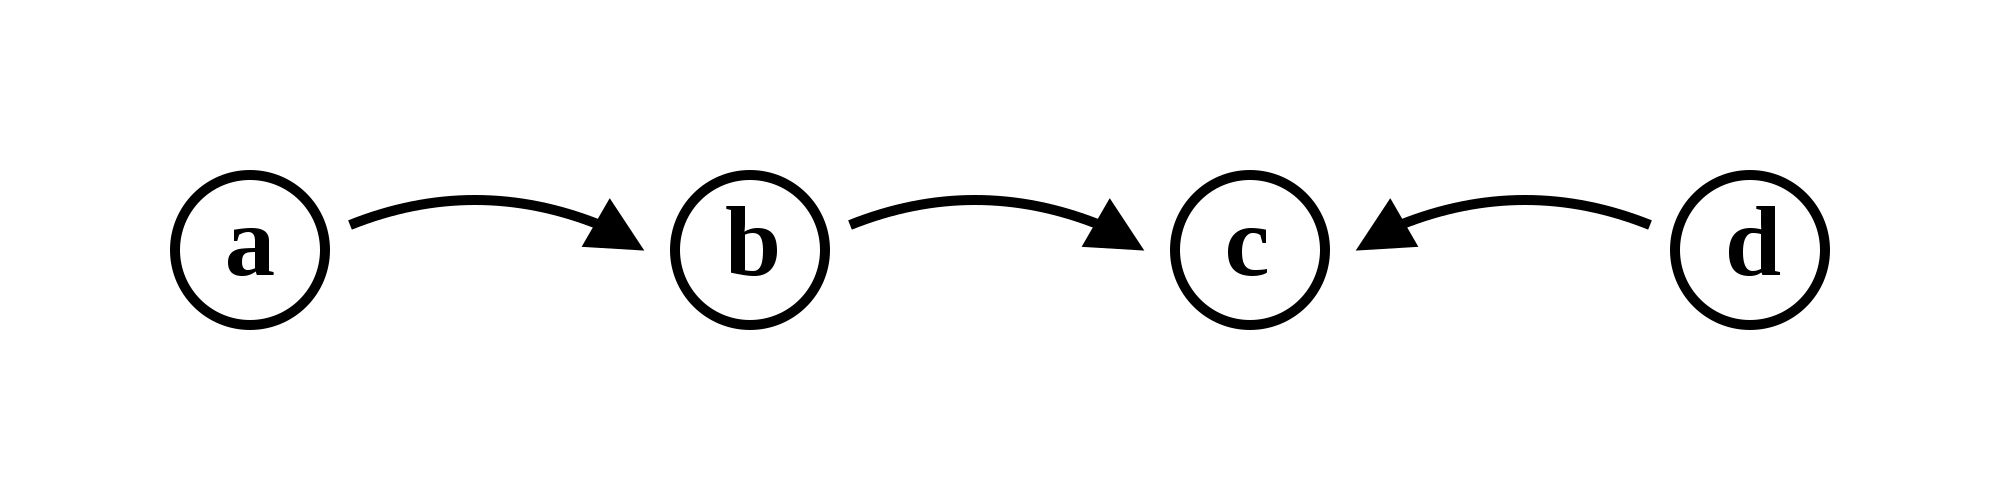
\includegraphics[width=\textwidth,keepaspectratio=true]{argumentationFramework.png}
	\caption{Representation fo argumentation framework, from \citep{argumentationFrameworkExample}}
	\label{fig:argumentationFrameworkFigure}
\end{figure}
 
Dung in his paper \citep{dung1995} has also defined notions of \textit{acceptable} and \textit{admissible} arguments, which are as follow:

\begin{definition}{Acceptable argument}
\label{AcceptableArgDef}\\
An argument \textit{a} $\in$ \textit{AR} is said to be \textit{acceptable} with respect to set \textit{S} $\subseteq$ \textit{AR} if and only if for each argument \textit{b} $\in$ \textit{AR} such that (\textit{b}, \textit{a}) $\in$ \textit{attacks}, there are some arguments \textit{c} $\in$ \textit{S} such that (\textit{c}, \textit{b}) $\in$ \textit{attacks}
\end{definition}

Hence it can be said that the argument from the argumentation framework is acceptable with respect to the set only if it is either conflict free, or there exists an argument from the same set that defends given argument. Based on the definition \ref{AcceptableArgDef}, definition of \textit{admissible} set can be concluded:

\begin{definition}{Admissible argument}
\label{AdmissibleArgDef}\\
A conflict-free set of arguments \textit{S} is \textit{admissible} if and only if each argument in \textit{S} is acceptable with respect to \textit{S}.
\end{definition}

\section{Argumentation Semantics}
That means that the set of arguments can be described as admissible only if it is conflict-free and all of its arguments can be defended by other arguments from that set. Both definitions have important role in defining the semantics of abstract argumentation. An argumentation semantics can be described as teh formal definition of a method (declarative or procedural) ruling the argument evaluation process \citep{baroni2009semantics}. Hence, they are used to evaluate if the arguments can be justified, by being defended by other arguments in the set, or rejected. There are two approaches for defining argumentation semantics: extension and labelling based. In the extension-based approach a semantics definition specifies how to derive from an argumentation framework a set of extensions, where an extension \textit{E} of an argumentation framework $<$\textit{AR, attacks}$>$ is simply a subset of \textit{AR}, intuitively representing a set of arguments which can “survive together” or are “collectively acceptable” \citep{baroni2009semantics}. On the other hand labelling-based approach defines how the arguments can be labelled based on the predefined set of labels. Labels define the possible states of argument and those are as follow: \textit{in}, when argument can be justified, \textit{out} when argument is rejected, and \textit{undecided} to any other argument. As shown by Modgil and Caminada, label-based approach is suitable for characterizing argumentation semantics \citep{modgil2009proof}.

The original concept of abstract argumentation semantics included complete, stable, preferred and grounded extensions \citep{dung1995}, which was extended by stage \citep{verheij1996two}, ideal \citep{dung2007computing}, and semi-stable \citep{caminada2006semi} semantics. All the sematics are based around the definitions of acceptable and admissible arguments. Definitions of the original semantics as described by \citet{dung1995} are as follow: 

\begin{definition}{Preferred Extension}
\label{def:preferredExtension}\\
A \textit{preferred extension} of an argumentation framework \textit{AF} is a maximal (with respect to set inclusion) admissible set of \textit{AF}.
\end{definition}

\begin{definition}{Stable Extension}
\label{def:stableExtension}\\
A \textit{conflict-free} set of arguments \textit{S} is called a \textit{stable extension} if and only if \textit{S} attacks each argument which does not belong to \textit{S}.
\end{definition}

\citet{dung1995} in his paper also defined a skeptical semantics known as grounded extension. This extension is defined in terms of \textit{characteristic function}, which in turn is defined as:

\begin{definition}{Characteristic Function}
\label{def:characteristicFunction}\\
The \textit{characteristic function}, denoted by \textit{F\textsubscript{AF}}, of an argumentation framework \textit{AF} = $<$\textit{AR, attacks}$>$ is defined as follows:
\[F_{AF}:2^{AR} \rightarrow 2^{AR}\]
\[F_{AF}(S)=\{A| \text{A is acceptable with respect to S} \}\]
\end{definition}

\begin{definition}{Grounded Extension}
\label{def:groundedExtension}\\
The \textit{grounded extension} of an argumentation framework \textit{AF}, denoted by \textit{GE\textsubscript{AF}}, is the least fixed point of \textit{F\textsubscript{AF}}.
\end{definition}

\begin{definition}{Complete Extension}
\label{def:completeExtension}\\
An admissible set \textit{S} of arguments is called \textit{complete exension} if and only if each argument which is acceptable with respect to \textit{S}, belongs to \textit{S}.
\end{definition}

Above semantics can be used to decide whether a given argument, or set of arguments can be accepted in terms of set inclusion.  Based on the definitions a number of inclusions between the sets can be conluded, which are:
\begin{itemize}
	\item{Grounded extension is the smallest complete extension}
	\item{Every preferred extesion is also complete}
	\item{Every stable extension is also preferred}
\end{itemize}
Furthermore, it can be seen that the maximal complete extension is also maximal admissible set.

As mentioned earlier, \citet{dung1995} semantics were further extended with additional semantics. 

\begin{definition}{Semi-stable extension}
\label{def:semiStableExtension}
Let (\textit{AR}, \textit{attacks}) be an argumentation framework and \textit{Args} $\subseteq$ \textit{AR}. \textit{Args} is called \textit{semi-stable extension} if and only if \textit{Args} is a complete extension where \textit{Args} $\cup$ \textit{$Args^+$} is maximal.
\end{definition}

\begin{figure}
\tikzset{
    main/.style={draw, rectangle, rounded corners, minimum height=1cm, minimum width=4.5cm},
    arrow/.style={thick,<-,>=stealth}
}
\centering
\begin{tikzpicture}[auto,node distance=1.5cm]
	\node[main](1){Complete Semantics};
	\coordinate[below=of 1](c);
  	\node[main](2)[left=of c]{Grounded Semantics};
  	\node[main](3)[right=of c]{Ideal Semantics};
  	\node[main](4)[below=of c]{Preferred Semantics};
  	\node[main](5)[below=of 4]{Semi-Stable Semantics};
  	\node[main](6)[below=of 5]{Stable Semantics};  	
  	%%% ARROWS %%%
  	\draw[arrow](1) -- (2);
  	\draw[arrow](1) -- (3);
  	\draw[arrow](1) -- (4);
  	\draw[arrow](4) -- (5);
  	\draw[arrow](5) -- (6);  	
\end{tikzpicture}
\caption{Relations of semantics}
\label{fig:semanticsRelations}
\end{figure}
